\documentclass[9pt]{beamer}
\usepackage{minted}
%\usemintedstyle{manni}
\usemintedstyle{murphy}
\usepackage{hyperref}
\hypersetup{
colorlinks=true,
urlcolor=blue
}
\usepackage{graphicx}

\begin{document}
\title{Securing Django Websites}
\author{Nick Thompson} 
\date{\today}

\frame{\titlepage}

\begin{frame}[fragile]
\frametitle{Getting started:}
\begin{minted}{bash}
$ git clone https://github.com/NAThompson/django_https.git
$ pyvenv django_https
$ cd django_https
$ pip3 install -r requirements.txt
$ sudo /bin/bash
$$ . bin/activate
\end{minted}
We'll need root to open up priviledged ports. Sourcing after acquisition of root shell is necessary.
\end{frame}

\begin{frame}
\frametitle{Server Stack}
\begin{itemize}
\item We're going to use Django+gunicorn+nginx to serve this website
\item \href{http://gunicorn.org/\#deployment}{gunicorn} is a web server gateway interface
\item We need nginx to reverse proxy because gunicorn is trivially vunerable to DOS attacks
\end{itemize}
\end{frame}

\begin{frame}[fragile]
\frametitle{Install nginx}
\begin{minted}{bash}
$ sudo apt-get install nginx # Ubuntu
$ sudo brew install nginx # Mac
\end{minted}
\end{frame}

\begin{frame}[fragile]
\frametitle{Symlink our nginx.conf into the global}
\begin{minted}{bash}
$ cd django_https
$ rm -f /etc/nginx/nginx.conf
$ rm -f /etc/nginx/sites-available/default
$ ln -s `pwd`/nginx.conf /etc/nginx/nginx.conf
$ ln -s `pwd`/default /etc/nginx/sites-available/default
\end{minted}
(Sorry peeps I didn't bother to relativize all the paths; you'll need to edit!)
\end{frame}

\begin{frame}[fragile]
\frametitle{How to serve the website}
\begin{minted}{bash}
$$ cd django_https/src
$$ gunicorn -c gunicorn_config.py https.wsgi &
$$ nginx
\end{minted}
(Again, there are some hard-coded paths in this . . .)
\end{frame}

\begin{frame}[fragile]
\frametitle{Redirects}
If we don't listen on port 80, then users will need to type the protocol into the browser, which no one does. 

Hence we need nginx to redirect:
\begin{minted}{bash}
server {
    listen         80;
    listen         [::]:80;
    server_name    www.example.com example.com;
    return         301 https://$server_name$request_uri;
}
\end{minted}
\end{frame}

\begin{frame}[fragile]
\frametitle{Turn SSL on and proxy-pass to gunicorn}
\begin{minted}{bash}
server {
  listen         443;
  ssl            on;
  server_name    example.com;
  ssl_certificate  /somedir/bundle.crt;
  ssl_certificate_key /somedir/mykey.key;

  location / {
     proxy_pass https://127.0.0.1:8000;
     proxy_set_header Host $host;
     proxy_set_header X-Forwarded-For $proxy_add_x_forwarded_for;
  }
}
\end{minted}
\end{frame}

\begin{frame}[fragile]
\frametitle{How secure is the default nginx configuration?}
\href{https://www.ssllabs.com/ssltest/analyze.html}{SSL Labs} doesn't think it's all that great:

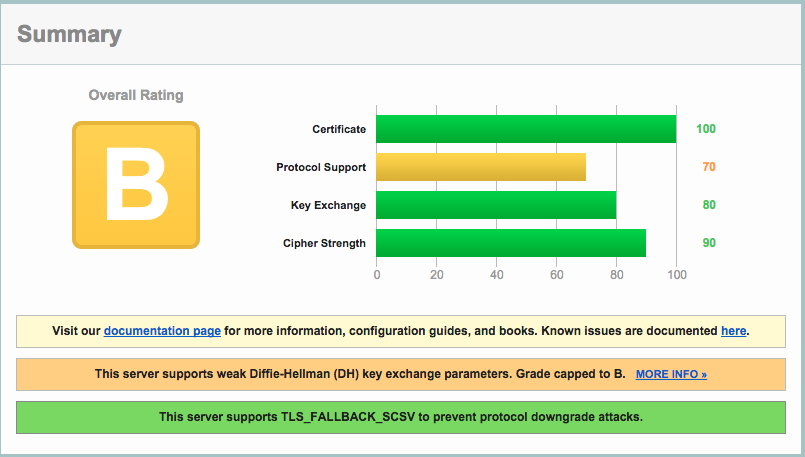
\includegraphics[scale=0.25]{figures/SSLLabsFirstGrade.png}
\end{frame}

\begin{frame}[fragile]
\frametitle{Improving SSLLabs grade}
In the nginx.conf, change 
\begin{minted}{c}
ssl_protocols TLSv1 TLSv1.1 TLSv1.2;
\end{minted}
to
\begin{minted}{c}
ssl_protocols TLSv1.2;
\end{minted}
Note: This will lose you some old IE browsers. SSLLabs will tell you which ones on their report.
\end{frame}

\begin{frame}
\frametitle{Some justification . . .}
\begin{itemize}
\item The \href{https://www.pcisecuritystandards.org/}{PCI Security Standards Council} says you must remove support for TLSv1.0 to be PCI compliant. ``SSL and early TLS are not considered strong cryptography and cannot be used as a security control after 30th June, 2016.``
\item \href{https://www.owasp.org/index.php/Transport_Layer_Protection_Cheat_Sheet}{OWASP} claims ``TLS 1.0 is still widely used as 'best' protocol by a lot of browsers, that are not patched to the very latest version. It suffers CBC Chaining attacks and Padding Oracle attacks. TLSv1.0 should only be used only after risk analysis and acceptance.``
\item Almost \href{https://en.wikipedia.org/wiki/Transport_Layer_Security\#Web_browsers}{no browsers} support TLSv1.1 and \emph{not} TLSv1.2. So make your life easier and just use 1.2.
\end{itemize}
\end{frame}

\begin{frame}[fragile]
\frametitle{Improving SSLLabs grade}
SSLLabs thinks that 256 bits symmetric protocols are better than 128 bit protocols, so we need to restrict the supported ciphers by adding this to the http section of nginx.conf:
\begin{minted}{c}
ssl_ciphers 'ECDHE-RSA-AES256-GCM-SHA384:ECDHE-ECDSA-AES256-GCM-SHA384:ECDHE-RSA\
-AES256-SHA384:ECDHE-ECDSA-AES256-SHA384:ECDHE-RSA-AES256-SHA:ECDHE-ECDSA-AES256-SHA:DHE\
-RSA-AES256-GCM-SHA384:DHE-RSA-AES256-GCM-SHA:DHE-RSA-AES256-SHA256:DHE-RSA-AES256-SHA:!\
aNULL:!eNULL:!LOW:!3DES:!MD5:!EXP:!PSK:!SRP:!DSS';
\end{minted}
This is a mess, what does it mean?
\end{frame}

\begin{frame}
\frametitle{This is called ciphersuite negotiation}
\begin{itemize}
\item The browser tells the server what cipher suites it supports
\item The server selects one that is in the ssl\_ciphers list,
\item The server tells the browser what ciphers they are using, or rejects the connection if they can't agree on a cipher suite.
\end{itemize}
\end{frame}

\begin{frame}
\frametitle{Interpreting ssl\_ciphers}
The order matters: Adding ``ssl\_prefer\_server\_ciphers on;`` to the nginx.conf tells nginx to ignore the preferences of the browser.

The order of entries to ssl\_ciphers tells nginx what cipher suite it should prefer.
\end{frame}

\begin{frame}[fragile]
\frametitle{Components of a ciphersuite}
\begin{itemize}
\item A key exchange algorithm (generally an asymmetric cipher, e.g. RSA)
\item An encryption algorithm (generally a symmetric cipher, e.g. AES)
\item A message authentication code algorithm  (hash function, SHA256)
\item A pseudo-random function
\end{itemize}
\end{frame}

\begin{frame}[fragile]
\frametitle{Understanding available ciphersuites}
To see what ciphers your nginx supports, run
\begin{minted}{bash}
$ openssl ciphers
\end{minted}
(nginx links against openssl)
\end{frame}

\begin{frame}[fragile]
\frametitle{Understanding available ciphersuites}
To understand a given cipher, we use
\begin{minted}{bash}
$ openssl ciphers -v 'ECDHE-RSA-AES256-GCM-SHA384'
ECDHE-RSA-AES256-GCM-SHA384 TLSv1.2 Kx=ECDH     Au=RSA  Enc=AESGCM(256) Mac=AEAD
\end{minted}
So ECDHE-RSA-AES256-GCM-SHA384 used elliptic curve Diffie-Helman for key exchange, RSA for authentication, 256 bit Advanced Encryption Standard in Galois Counter mode for encryption, and ``authentication encryption with associated data'' for message authentication.
\end{frame}

\begin{frame}
\frametitle{What ciphersuites does my browser support?}
There are \href{https://cc.dcsec.uni-hannover.de/}{some websites} who will tell you:
\begin{figure}
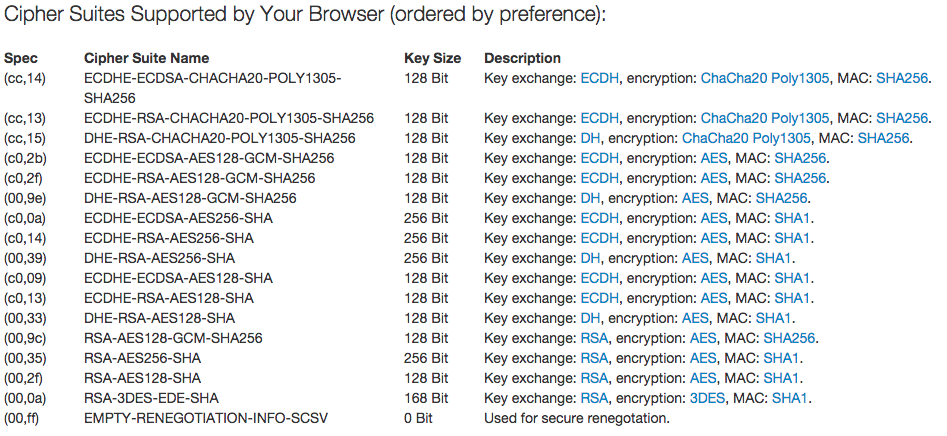
\includegraphics[scale=0.25]{figures/browserciphersuites.png}
\end{figure}
\end{frame}

\begin{frame}[fragile]
\frametitle{SSLLabs thinks 256 bit bulk encryption with SHA-256 or greater is neat:}
So let's try this:
\begin{minted}{bash}
ssl_ciphers = 'ECDHE-ECDSA-AES128-GCM-SHA256:
                   ECDHE-RSA-AES128-GCM-SHA256:
                   DHE-RSA-AES128-GCM-SHA256:
                   ECDHE-ECDSA-AES256-SHA:
                   ECDHE-RSA-AES256-SHA:
                   DHE-RSA-AES256-SHA:
                   ECDHE-ECDSA-AES128-SHA:
                   ECDHE-RSA-AES128-SHA:
                   DHE-RSA-AES128-SHA:
                   RSA-AES128-GCM-SHA256:
                   RSA-AES256-SHA';   
\end{minted}
\end{frame}

\begin{frame}
\frametitle{Some advice:}
\begin{itemize}
\item \href{https://www.schneier.com/blog/archives/2009/07/another_new_aes.html}{Prefer} 128-bit AES to 256-bit AES
\item Prefer Galois counter modes as they consume less resources
\item Prefer SHA256 over SHA1 as SHA1 will be \href{http://googleonlinesecurity.blogspot.com/2014/09/gradually-sunsetting-sha-1.html}{deprecated}.
\item \href{https://www.nsa.gov/business/programs/elliptic_curve.shtml}{Prefer} elliptic curves, unless you think the NSA has a \href{https://en.wikipedia.org/wiki/Elliptic_curve_cryptography}{quantum computer}.
\end{itemize}
\end{frame}

\begin{frame}[fragile]
\frametitle{Enabling Perfect-Forward Secrecy}
 ``. . . which \href{https://www.owasp.org/index.php/Transport_Layer_Protection_Cheat_Sheet}{means} a compromise of the server's long term signing key does not compromise the confidentiality of past session''
 
 We can get perfect forward secrecy via use of ephemeral keys . . .
\end{frame}

\begin{frame}[fragile]
To use ephemeral keys we need to generate big primes:
\begin{minted}{bash}
$ openssl dhparam -out dhparam.pem 4096
\end{minted}
and add the following line to the nginx.conf:
\begin{minted}{bash}
ssl_dhparam /path_to_pem/dhparam.pem
\end{minted}
\end{frame}

\begin{frame}[fragile]
\frametitle{SSLLabs is now Happy}
\begin{figure}
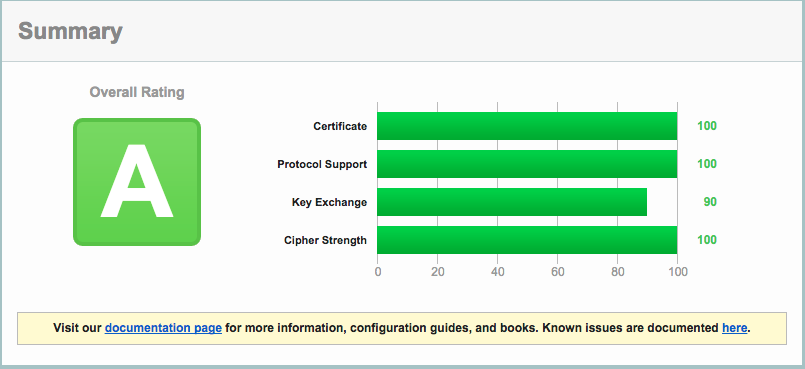
\includegraphics[scale=0.25]{figures/SSLLabsA.png}
\end{figure}
You can see the SSLLabs rating guide \href{https://www.ssllabs.com/downloads/SSL_Server_Rating_Guide.pdf}{here}.
\end{frame}

\begin{frame}[fragile]
\frametitle{But there's still low-hanging fruit!}
Add this to the server section in default:
\begin{minted}{c}
add_header Strict-Transport-Security "max-age=63072000; includeSubdomains";
\end{minted}
\begin{figure}
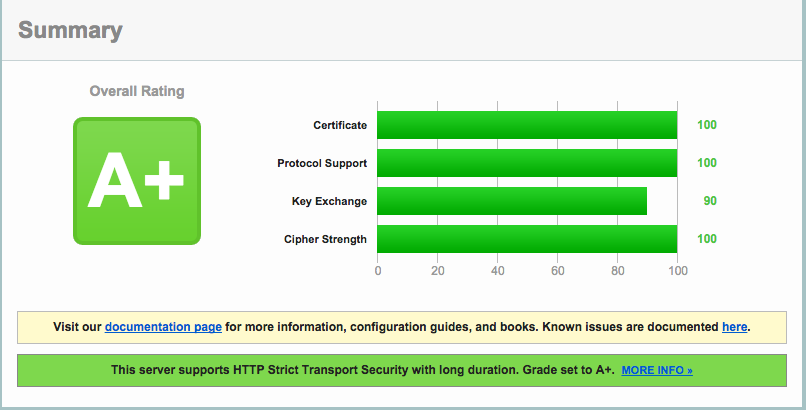
\includegraphics[scale=0.25]{figures/SSLLabsAp.png}
\end{figure}
\end{frame}

\begin{frame}[fragile]
\frametitle{What is Strict Transport Security?}
\begin{itemize}
\item A protocol by which servers force all traffic to come over https.
\item Stops downgrade attacks and cookie hijacking.
\item max-age is the period over which browsers should remember to come to that server with only https requests
\end{itemize}
\end{frame}

\begin{frame}[fragile]
\frametitle{What is Strict Transport Security?}
A user who has visited your site previously \emph{cannot} proceed past a bad certificate:
\begin{figure}
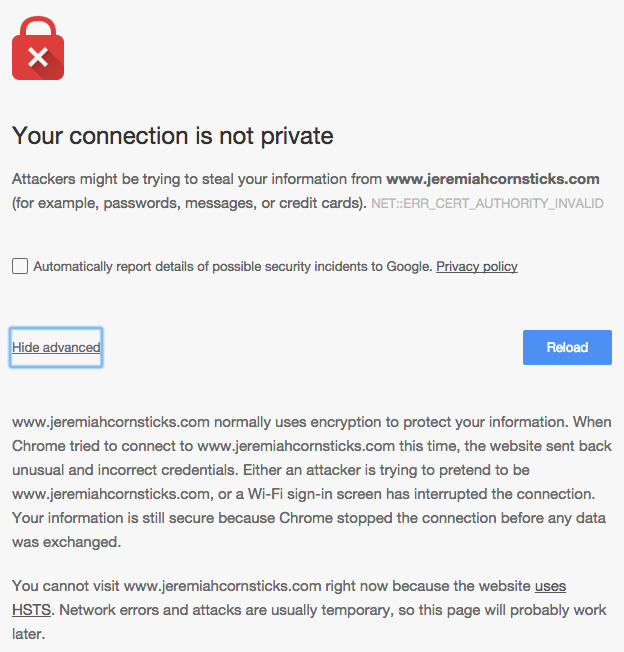
\includegraphics[scale=0.25]{figures/HSTSNoRedirect.png}
\end{figure}
(Unless they clear their browser cache . . . then the user can ignore the warning and proceed.)
\end{frame}

\begin{frame}[fragile]
\frametitle{HSTS Redirects http to https}
\emph{But only after a user visits the first time . . .}

Workaround:

Register your site in the \href{https://hstspreload.appspot.com/}{preload list!}

``This form is used to submit domains for inclusion in Chrome's HTTP Strict Transport Security (HSTS) preload list. This is a list of sites that are hardcoded into Chrome as being HTTPS only.''
\end{frame}

\begin{frame}[fragile]
\frametitle{Most importantly!}
HSTS prevents \href{http://www.thoughtcrime.org/software/sslstrip/}{SSL stripping!} 
\end{frame}


\begin{frame}[fragile]
\frametitle{Last one!}
To get a strong key-exchange, we need at least 4096 bit keys:
\begin{minted}{bash}
$ openssl genrsa -out foo.key 4096
$ openssl req -new -sha256 -key foo.key -out foo.csr
\end{minted}
Use this certificate signing request to get certs from your provider, and you're done!
\begin{figure}
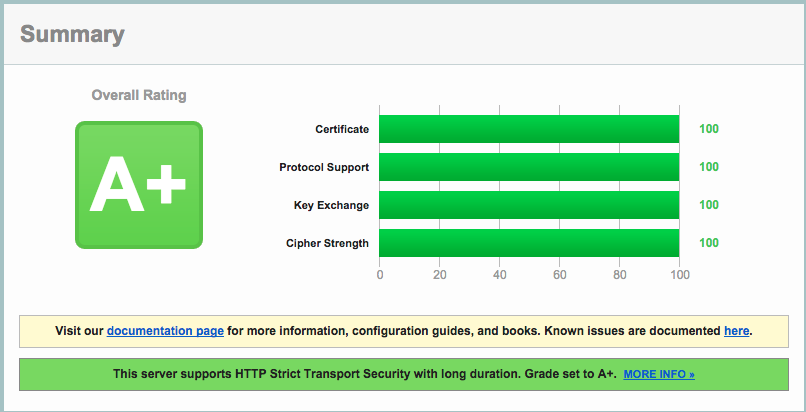
\includegraphics[scale=0.25]{figures/App.png}
\end{figure}
\end{frame}

\begin{frame}[fragile]
\frametitle{OCSP Stapling}
\begin{itemize}
\item OCSP := Online Certificate Status Protocol
\item Used to determine if a certificate has been revoked
\item Browsers must query CA, revealing websites they visit
\item OCSP Stapling: Server caches CA's OCSP response, increasing privacy as well as speed
\end{itemize}
\end{frame}

\begin{frame}[fragile]
\frametitle{Clickjacking}
\begin{itemize}
\item Someone renders your page in theirs (example: ebay.com/buynicecar)
\item Then they make your page invisible, but put ``Win free iPad!'', and a place to click over the ``Buy it now'' link of the ebay listing
\item If you are logged in on ebay, you are the proud owner of a new car!
\end{itemize}
\end{frame}

\begin{frame}
\frametitle{Clickjacking}
``\href{https://www.owasp.org/index.php/Clickjacking}{One} of the most notorious examples of Clickjacking was an attack against the Adobe Flash plugin settings page. By loading this page into an invisible iframe, an attacker could trick a user into altering the security settings of Flash, giving permission for any Flash animation to utilize the computer's microphone and camera.''
\end{frame}

\begin{frame}
\frametitle{Defense against clickjacking}
As a web user: You're screwed.
\end{frame}

\begin{frame}[fragile]
\frametitle{Defense against clickjacking}

As a developer: Add the following to your nginx.conf:
\begin{minted}{c}
add_header X-Frame-Options DENY;
\end{minted}
Note that this was a non-standard extension to html. There is a standardized way, but it's not yet supported by all modern browsers
\end{frame}



\end{document}
